\chapter{Analisi Associativa}

Di seguito verrà descritto il lavoor svolto nell'ambito della ricerca di regole associative esistenti fra i dati che abbiamo appositamente processato. \\

Come è già stato accennato in precedenza, questo tipo di analisi è stata messa in atto sulle versioni discretizzate dei data set. Il motivo di questo requisito apparirà chiaro andando a descrivere nel dettaglio il funzionamento delle tecniche di analisi associativa.

\section{Introduzione all'analisi associativa}

    \subsection{Regole Associative}

        Una regola associativa è una implicazione del tipo $A \rightarrow B$, con $A$ e $B$ insiemi di item (detti, appunto \textit{itemset}). Il significato di ciò dovrebbe essere palese: data la presenza di $A$ in una istanza del data set, è \textit{fortemente probaible} la presenza di $B$. La valutazione di questa probaiblità avviene considerando alcune metriche particolari quali, ad esempio, la \textit{confidenza} o il \textit{lift}. \\

        Portando un esempio sul dataset oggetto di questa analisi, una tanto probabile quanto banale regola associativa che ci si aspetta di trovare potrà essere del tipo \textit{"Valutazione del corso: ALTA"} $\rightarrow$ \textit{"Voto conseguito: ALTO"}. \\
        
        Quello a cui si mira, però, è il riuscire a scoprire qualche altra regola che trascenda il limite dell'ovvio, aprendo così le porte a interpretazioni non immediate dell'insieme di dati su cui si sta lavorando. Per questo motivo, oltre all'aiuto di criteri algoritmici di potatura, occorrerà comunque prevedere un \textit{intervento umano} nel \textit{post processing} delle regole generate.

    \subsection{L'algoritmo Apriori di Weka}

    \begin{figure}
        \centering
        \caption{pannello di scelta delle impostazioni per l'algoritmo Apriori di Weka}
        \label{apriori_weka}
	    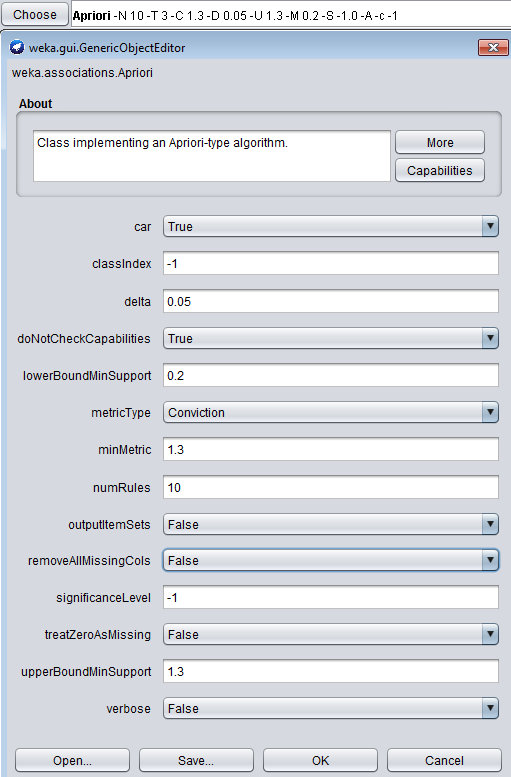
\includegraphics[scale=0.7]{img/apriori_weka.png}
    \end{figure}

        Il processo di generazione delle regole associative utilizzato in questa analisi si basa sul \textbf{principio Apriori}. Dato da una regola non è altro che una implicazione fra due itemset che compaiono frequentemente insieme, e che quindi compaiono co una certa frequenza anche da soli, il pilastro fondamentale da cui partire per generare le regole è il \textit{mining} degli itemset frequenti. \\
        
        In estrema sintesi, l'idea generale è quella di generare una lista di \textit{candidati} semplici --- cioè di itemset che potrebbero essere frequenti --- verificarne il \textit{supporto} e usare quelli frequenti per generare altri candidati più complessi. Il principio Apriori, infatti, stabilisce che se un itemset con pochi elementi è infrequente, lo saranno anche tutti gli itemset che lo comprendono. Questo fatto, detto \textit{anti-motonia} del supporto, ci consente di evitare di generare e calcolare la frequenza di ogni possibile itemset, rendendo trattabile quello che sarebbe invece un problema $NP-Completo$. \\

        Nel dettaglio dell'analisi da effettuare, l'algoritmo Apriori messo a disposizione dal software Weka accetta in input diversi parametri, che consentono di specificarne il comportamento dell'algoritmo, adattandolo agli scopi che ci si è prefissi. Si veda adesso una configurazione di esempio:\\

        \begin{center}
            \noindent \texttt{Apriori -N 10 -T 0 -C 0.9 -D 0.05 -U 1.0 -M 0.1}
        \end{center}

        I vari \textit{flags} da passare come argomenti vanno a regolare questi parametri della computazione:

        \begin{itemize}
            \item \texttt{-N}: numero di regole associative da trovare
            \item \texttt{-T}: tipo di metrica utilizzata per la valutazione degli itemset.
                \subitem 0 - \textit{confidence}
                \subitem 1 - \textit{lift}
                \subitem 2 - \textit{leverage}
                \subitem 3 - \textit{convction}
            \item \texttt{-C}: valore minimo della metrica indicata per considerare frequente un itemset
            \item \texttt{-D}: valore che viene usato per diminuire il supporto ad ogni iterazione dell'algoritmo
            \item \texttt{-U}: limite superiore del supporto minimo richiesto
            \item \texttt{-M}: limite inferiore del supporto minimo richiesto 
        \end{itemize}

        Ovviamente, come si può vedere in \ref{apriori_weka}, sono possibili molte altre personalizzazioni e impostazioni, fatto che rende l'implementazione di Weka dell'algoritmo Apriori estremamente flessibile ed adattabile a molte esigenze.
 
\section{Apriori su dataset aggregato}

    Lorem ipsum ecc

        \subsection{Focus sul corso}

            \lstinputlisting{../ass/apriori_min_1.txt}

        \subsection{Focus sul docente}

            \lstinputlisting{../ass/apriori_min_2.txt}

        \subsection{Focus sulla Deviazione Standard}

            \lstinputlisting{../ass/apriori_min_3.txt}
